\section{Introduction}
\label{sec:introduction}

\todo{Introduction goes here.}

\todo{We motivate the problem of deciding serializability in programmable networks.}

\todo{We talk about some related work if relevant.}

\todo{We show that it's interesting with an example.}

\todo{We describe our main results.}

\paragraph{Contributions:}
\begin{itemize}
    \item Novel notion of serializability (``atomicity'' or ``semantic serializabillity'') applicable to network systems (\Cref{sec:problem-definition,sec:related:notions-of-serializability})
    \item Decidability results (1 main theorem: \textbf{automatically proving unbounded serializability}, 2 extra theorems: ser=ser decidable, ser=int undecidable) (\Cref{sec:formal-results,sec:related:deciding-serializability})
    \item Implementation of decision procedure. Advances in semilinear sets, Petri net reachability heuristics that makes the decision procedure work. (\Cref{sec:implementation,sec:related:petri})
\end{itemize}

\newpage


\paragraph{Motivation:}

example - 1

	
	
\noindent
\begin{minipage}[t]{0.45\textwidth}
	\begin{minipage}[t]{\textwidth}
		\begin{lstlisting}[caption={Without yield or lock (serializable)}]
    request foo: 
        X := 1 
        // no yield
        y := X 
        X := 0
        return y 
		\end{lstlisting}
	\end{minipage}
	\vspace{1em}
	\begin{minipage}[t]{\textwidth}
		\begin{lstlisting}[caption={With yield (not serializable)}]
    request foo: 
        X := 1 
        yield 
        y := X + 1
        X := 0
        return y 	
		\end{lstlisting}
	\end{minipage}
\end{minipage}%
\hfill
\begin{minipage}[t]{0.45\textwidth}
	\begin{lstlisting}[caption={With yield and lock (serializable)}]
    request foo: 
        // lock
        while (L == 1): 
            yield
        L := 1 

        X := 1
        yield
        y := X 
        X := 0

        // unlock    
        L := 0
        return y 
	\end{lstlisting}
\end{minipage}

\vspace{2em}
example - 2

% Second row
\noindent
\begin{minipage}[t]{0.45\textwidth}
	\begin{lstlisting}[caption={Not serializable: {(A,0),(A,0)}}]
		request A: 
		    x := FLAG 
		
		    if (?): 
		        yield
		    // no else
		
		
		    FLAG := 1 
		    return x
	\end{lstlisting}
\end{minipage}%
\hfill
\begin{minipage}[t]{0.45\textwidth}
	\begin{lstlisting}[caption={Serializable}]
		request A: 
		    x := FLAG
		
		    if (?):
		        yield
		    else:
		        x := 1 - x
		
		    FLAG := 1
		    return x
	\end{lstlisting}
\end{minipage}

\vspace{2em}
\newpage
example - 3

% Third row
\noindent
\begin{minipage}[t]{0.45\textwidth}
	\begin{lstlisting}[caption={Fred (serializable)}]
		request incr: 
		    while (X == 3):
		        yield
		        
		        
		    X := X + 1
		
		
		request decr: 
		    while (X == 0): 
		        yield
		        
		        
		    X := X - 1
	\end{lstlisting}
\end{minipage}
\hfill
\begin{minipage}[t]{0.45\textwidth}
	\begin{lstlisting}[caption={Fred2 (not serializable)}]
		request incr:
		    while (X == 3):
		        yield
		    y := X
		    yield
		    X := y + 1
		
		
		request decr: 
		    while (X == 0):
		        yield
		    y := X
		    yield
		    X := y - 1
	\end{lstlisting}
\end{minipage}
	

example - 4

\begin{minipage}[t]{1.0\textwidth}
\begin{lstlisting}[caption={Snapshot-based monitor deactivation (not serializable, as it can return a sume of 0 active monitors)}]
	// initialize both monitors to be active
    N_1_ACTIVE := 1
    N_2_ACTIVE := 1
	
    request main:
        // take snapshot
        n_1_active_snapshot := N_1_ACTIVE
        n_2_active_snapshot := N_2_ACTIVE
        yield
		
        if (n_1_active_snapshot == 1) and (n_2_active_snapshot == 1):
            // if both nodes active --- choose which one to deactivate 
            if (?): 
                N_1_ACTIVE := 0
            else:
                N_2_ACTIVE := 0

        return N_1_ACTIVE + N_2_ACTIVE  // total active nodes
\end{lstlisting}
\end{minipage}
	
%only 0 in non-serializable runs!

\newpage

example - 5

\noindent
\begin{minipage}[t]{0.45\textwidth}
	\begin{lstlisting}[caption={bank (serializable)}]
    // initialize accounts
    A := 100
    B := 50
    
    request transfer: 
        // transfer 50$
        A := A - 50
        // no yield
        B := B + 50
        return A + B
			
    request interest: 
        // add a 100% interest
        A := A + A
        // no yield
        B := B + B
        return A + B	      		        
		\end{lstlisting}
\end{minipage}
\hfill
\begin{minipage}[t]{0.45\textwidth}
	\begin{lstlisting}[caption={bank with yields (non serializable)}]
    // initialize accounts
    A := 100
    B := 50
		
    request transfer: 
        // transfer 50$
        A := A - 50
        yield
        B := B + 50
        return A + B

    request interest: 
        // add a 100% interest
        A := A + A
        yield
        B := B + B
        return A + B	      		        
	\end{lstlisting}
\end{minipage}
	
%\newpage


example - 6


% Second row
\noindent
\begin{minipage}[t]{0.45\textwidth}
	\begin{lstlisting}[caption={Complex while (serializable)}]
    request flip: 
        X := 1 - X 
    
    request main:
        i := 5
        while (i > 0):
            while (X == 0):
                pass
            while (X == 1):
                pass
            i := i - 1
        
        return 1       
		\end{lstlisting}
\end{minipage}%
\hfill
\begin{minipage}[t]{0.45\textwidth}
	\begin{lstlisting}[caption={Complex while with yields (not serializable)}]
    request flip: 
        X := 1 - X 

    request main:
        i := 5
        while (i > 0):
            while (X == 0):
                yield
            while (X == 1):
                yield
            i := i - 1

        return 1        
			\end{lstlisting}
\end{minipage}



\newpage

example - 7

\begin{minipage}[t]{1.0\textwidth}
	\begin{lstlisting}[caption={BGP (non serializable --- cycles can appear)}]
    // initialize accounts
    G := 0
    
    request policy_update:
    if (?):
        G := 1  // green policy 
    else:
        G := 0 // red policy
		
    request route_from_west:
        visited_east := 0
        current := 1
        while (current == 2) or (current == 3): // still routing        
            if (current == 1): // west (switch 1)
                if (G == 1): // green policy
                    current := 2
                else: // red policy
                    current := 1
            if (current == 2): // east (switch 2)
                visited_east := 1
                if (G == 1): // green policy
                    current := 3
                else: // red policy
                    current := 1
 
            yield
		
        return current + current + visited_east
        
    request route_from_east:
        ... // dual case     		        
	\end{lstlisting}
\end{minipage}


%// [WEST, switch 1] ---> [EAST, switch 2] ---> [out, switch 3] 
%else:
%G := 0 // red policy
%// [out, switch 0] <--- [WEST, switch 1] <--- [EAST, switch 2] 

\begin{figure}[h]
	\centering
	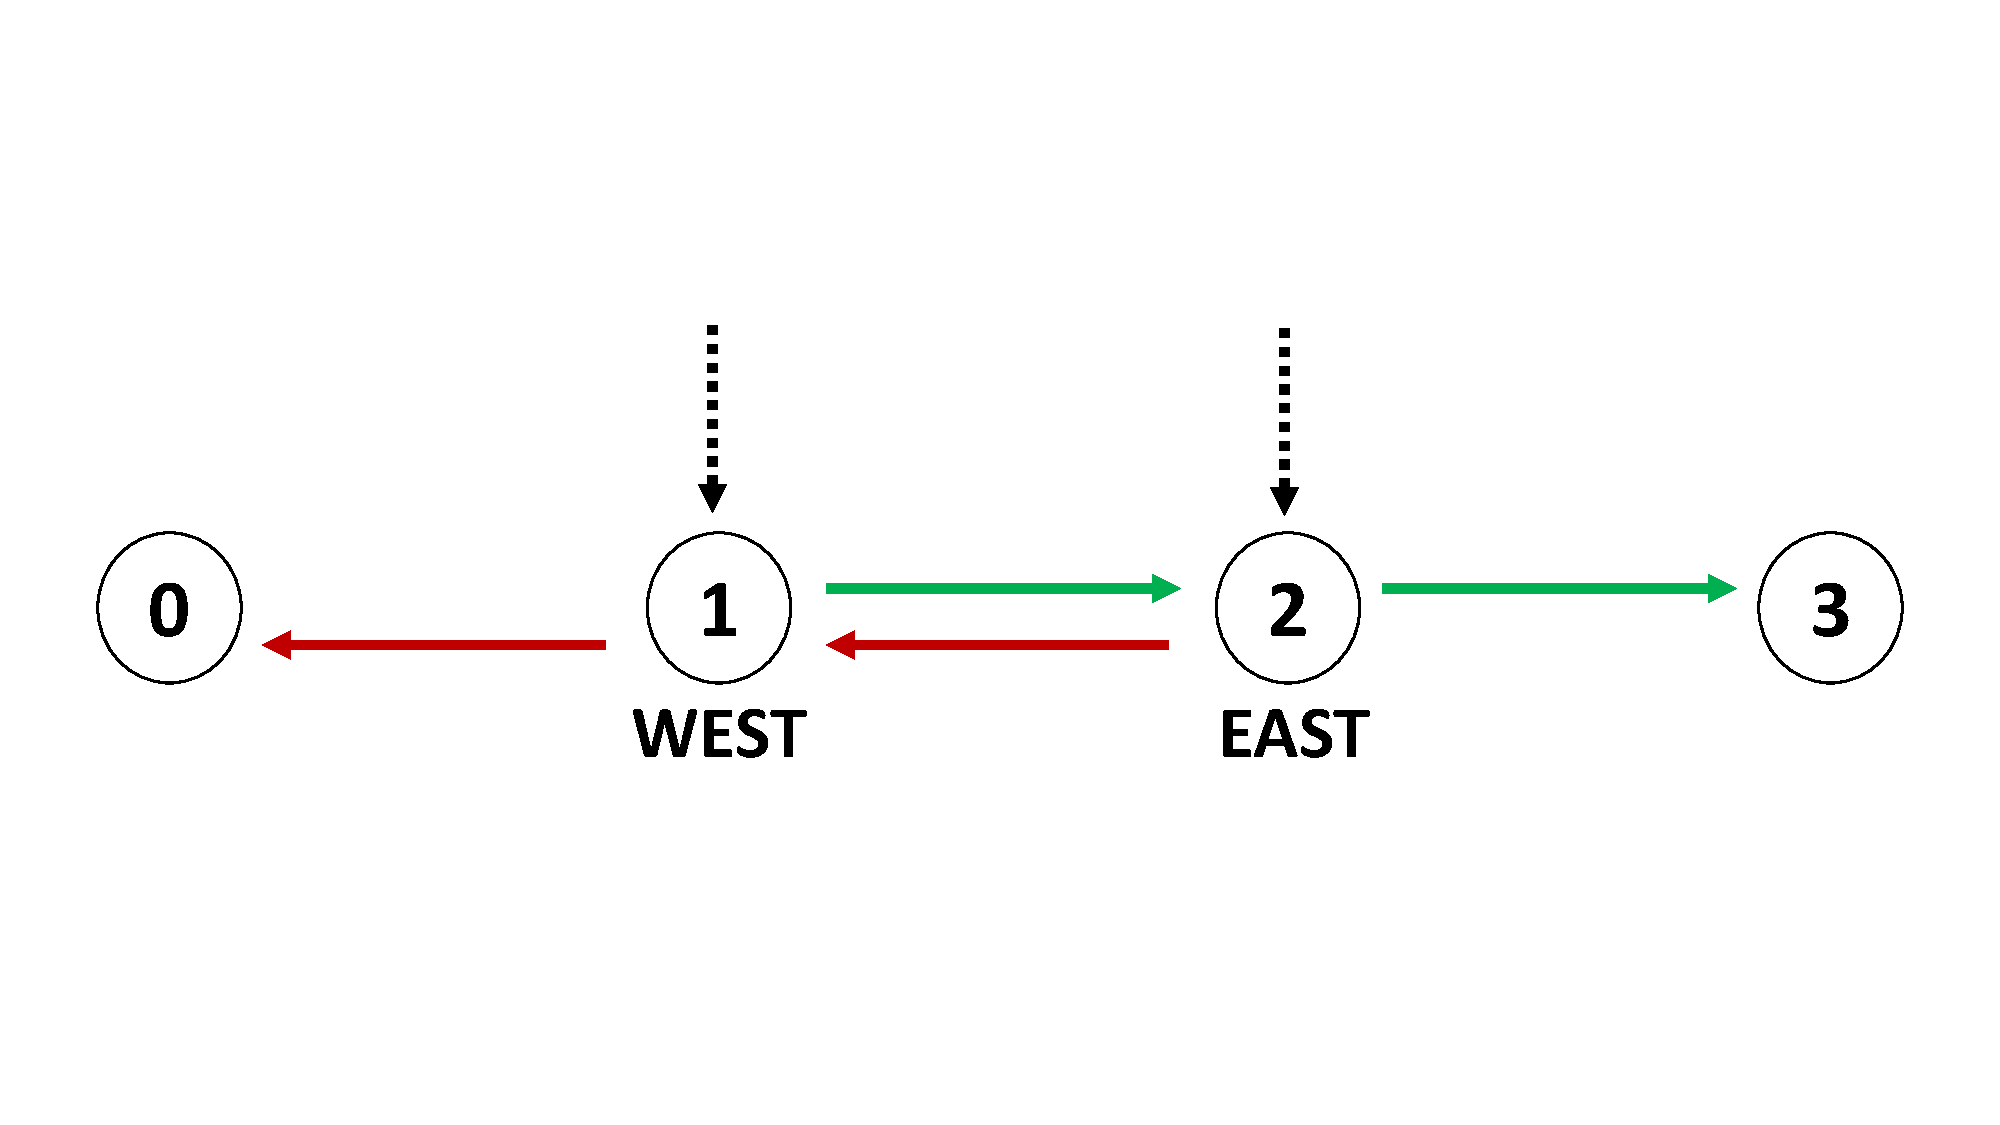
\includegraphics[width=0.65\linewidth]{plots/BgpColoredRouting.pdf}
	\caption{Routing policy in example 7.}
	\label{fig:pdfimage}
\end{figure}

\newpage